\documentclass[a4paper,12pt]{article}
\usepackage[utf8]{inputenc}
\usepackage[spanish]{babel}
\usepackage{amsmath, amssymb}
\usepackage{graphicx}
\usepackage{geometry}
\usepackage{hyperref}
\usepackage{float}
\usepackage{fancyhdr}
\usepackage{tocloft}
\usepackage{caption}
\captionsetup[figure]{skip=2pt}
\geometry{margin=2.5cm}

% Encabezado y pie de página
\pagestyle{fancy}
\fancyhf{}
\lhead{Inferencia y Estimación}
\rhead{Universidad de San Andrés}
\cfoot{\thepage}

% Numeración automática de figuras y formato uniforme
\renewcommand{\thefigure}{\arabic{figure}}
\captionsetup[figure]{skip=2pt, labelfont=bf, labelsep=period}

% Portada formal
\begin{document}
\noindent
\begin{minipage}{\textwidth}
    \centering
    {\scshape\LARGE Universidad de San Andrés \par}
    \vspace{1.2cm}
    {\scshape\Large Inferencia y Estimación\par}
    \vspace{1.2cm}
    {\huge\bfseries Compresión y Descompresión de Imágenes usando PCA\par}
    \vspace{1.5cm}
    {\large
    Catalina Hirsch - 36557 \\ Clara Zavaroni Benoit - 36772 \\ Maylen Antonella Villagrán Cardozo - 36758 \\}
    \vspace{1cm}
    {\large \today\par}
\end{minipage}



\begin{abstract}
La realización de este trabajo práctico tiene como objetivo aplicar el método de \textbf{Análisis de Componentes Principales (PCA)} en la compresión de imágenes. 
Se busca reducir el espacio de almacenamiento minimizando la pérdida de información, conservando los datos que contienen la mayor parte de la varianza. 
Posteriormente, se descomprime la imagen y se compara con la original para evaluar la calidad de la compresión, utilizando métricas objetivas. 
El desempeño se evalúa en función de la cantidad de componentes principales utilizados. A pesar de ciertos inconvenientes atravesados con las librerías utilizadas para programar,
lo cuál fue solucionado con la investigación acerca de ellas, no nos encontramos con mayores dificultades.
En primer lugar, se analizó la correlación entre píxeles contiguos de una imagen, presentando una alta correlación ($\approx 1$) en la imagen con mayor suavidad.
A comparación con otra imagen, con una mayor cantidad de ruido, en la cual obtuvimos una correlación más baja ($\approx 0.2$).
Luego, llevó a el proceso de compresión y descompresión, utilizando el método de PCA. 
En los resultados obtenidos, se puede observar el uso de la reducción de la la dimensionalidad en el ahorro almacenamiento, evitando comprometer la calidad la imagen.
Se encuentra demostrado posteriormente, donde aumentar la cantidad de espacio ahorrado, la cantidad de de componentes principales disminuye,
causando una disminución la calidad de la visualmente.
\end{abstract}



\newpage
\section*{Introducción}
\addcontentsline{toc}{subsection}{Introducción}
El objetivo de este trabajo práctico es implementar y evaluar la compresión y descompresión de imágenes utilizando el método de Análisis de Componentes Principales (PCA).
Para poder aplicar el método de PCA, en primer instancia fue necesario convertir los datos de la imagen en una matriz:
\begin{equation}
M \in \mathbb{R}^{m \times n}
\label{eq:matrizM}
\end{equation}
en donde cada fila corresponde a una muestra, obteniendo $\mathbf{x}_1, \mathbf{x}_2, \ldots, \mathbf{x}_m$, con $\mathbf{x}_i \in \mathbb{R}^{n \times 1}$.

Además, se calcula la media de las $\mathbf{x}_i$, con el fin de centrar los datos:
\begin{equation}
\boldsymbol{\mu}_x = \frac{1}{m} \sum_{k=1}^m \mathbf{x}_{k}
\label{eq:media}
\end{equation}
Obteniendo de esta forma el vector de media $\boldsymbol{\mu}_x \in \mathbb{R}^{n \times 1}$, que contiene el promedio de cada columna de $M$.

Luego se centra la matriz de datos restando la media a cada fila, obteniendo así la matriz centrada:
\begin{equation}
X_c = X - \mathbf{1}_m \boldsymbol{\mu}_x^T
\label{eq:centrado}
\end{equation}
Por como están los datos en la matriz $X$, la media se resta a cada fila, es decir, a cada bloque, usando el vector columna de unos $\mathbf{1}_m$.

Además, calculamos la matriz de covarianza $C_X$, que describe cómo varían conjuntamente las distintas posiciones dentro de los bloques. 
\begin{equation}
C_X = \frac{1}{m-1} X_c^T X_c
\label{eq:covarianza}
\end{equation}
Cada elemento $c_{ij}$ de $C_X$ representa la covarianza entre la posición $i$ y la posición $j$ dentro de los bloques.

Para aplicar PCA, se resuelve el problema de autovalores y autovectores de la matriz de covarianza.
Así es como se obtiene $P$ la matriz de autovectores, y $\lambda$ los autovalores asociados. Los cuales son ordenados, para luego seleccionar los $k$ más grandes, que corresponden a las direcciones de mayor varianza en los datos. Los autovectores asociados se agrupan en la matriz de proyección:
\begin{equation}
P = \begin{bmatrix}
| & | &        & | \\
\mathbf{p}_1 & \mathbf{p}_2 & \cdots & \mathbf{p}_k \\
| & | &        & |
\end{bmatrix}
\label{eq:autovectores}
\end{equation}

Finalmente, se define la transformación de PCA de la siguiente manera:
\begin{equation}
Y = X_c P
\label{eq:pca}
\end{equation}
Donde $P$ proyecta los datos originales sobre este subespacio de menor dimensión, resultando en la matriz $Y$ de datos comprimidos y descorrelacionados. Así, $Y \in \mathbb{R}^{m \times k}$, donde cada fila es la representación comprimida de cada bloque original $\mathbf{y}_i \in \mathbb{R}^{k \times 1}$.

Para la instancia de reconstrucción, se almacenan la matriz $Y$ de datos comprimidos, la matriz de autovectores $P$ y el vector de medias $\boldsymbol{\mu}_x$. La reconstrucción aproximada de la imagen original se realiza aplicando la transformación inversa:
\begin{equation}
\hat{X} = Y P^T + \mathbf{1}_m \boldsymbol{\mu}_x^T
\label{eq:reconstruccion}
\end{equation}

Para poder seleccionar el número de componentes principales $k$ a conservar, se define el porcentaje de espacio ahorrado $S$ como:
\begin{equation}
S = \left( 1 - \frac{\text{cantidad de componentes principales } (k)}{\text{cantidad de componentes totales } (m)} \right) \times 100 \%
\label{eq:espacio}
\end{equation}

El rendimiento del procedimiento se evalúa calculando el error cuadrático medio (MSE) entre la imagen original y la reconstruida. 
\begin{equation}
MSE = \frac{1}{N_w N_h} \sum_{i=1}^{N_w} \sum_{j=1}^{N_h} (p_{ij} - \hat{p}_{ij})^2
\label{eq:mse}
\end{equation}

\newpage

\section{Resultados y discusion:}
\subsection*{Ejercicio 1: Correlación}
\addcontentsline{toc}{subsection}{Ejercicio 1: Correlación}
El propósito de este ejercicio es analizar el comportamiento de los píxeles vecinos en las imágenes utilizadas. En primer lugar, se cargan las imágenes y se convierten a escala de grises. Luego, se divide cada imagen en bloques de 2x1 píxeles contiguos verticalmente. A continuación, se calcula la correlación entre los píxeles de cada bloque y se almacena en un vector. Finalmente, se realiza un gráfico de dispersión de las correlaciones obtenidas para cada imagen. Los resultados se presentan a continuación:


\begin{figure}[H]
    \centering
    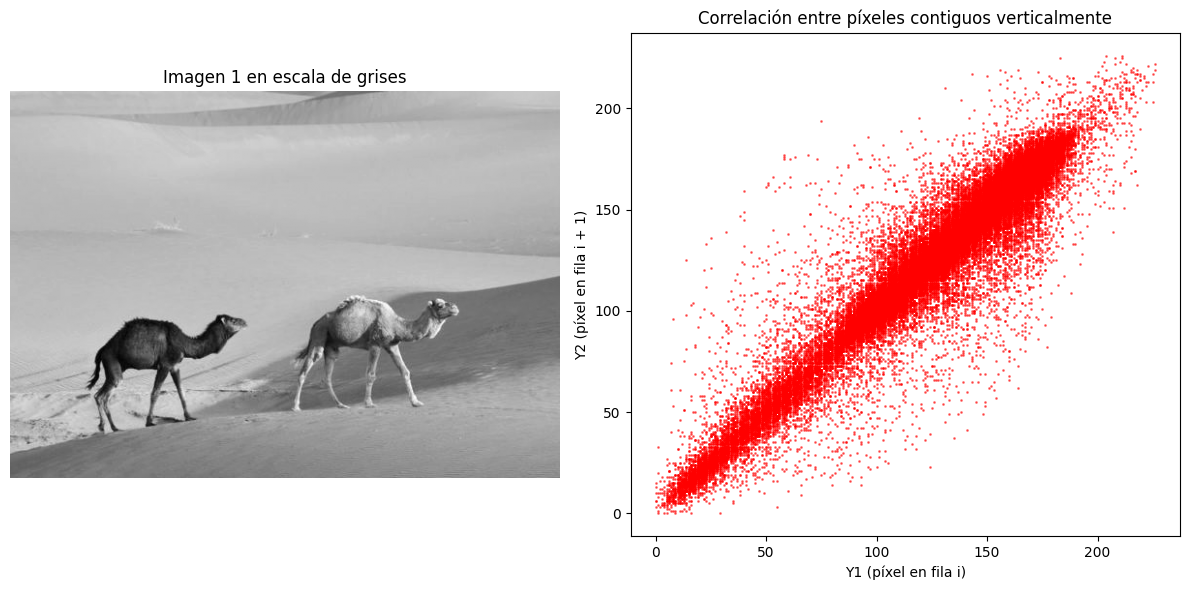
\includegraphics[width=1\textwidth]{Ejercicio1a.png}
        \caption{Gráfico de dispersión de la correlación de píxeles contiguos verticalmente de la imagen 1. 
    Se observa que los puntos se alinean en torno a una recta creciente. Es el resultado que esperabamos
    ya que los pixeles vecinos tienen colores similares.}
    
    \captionsetup{belowskip=0pt}
\end{figure}
\vspace{-1em}
Analizando el comportamiento del gráfico, la alineacion de los puntos indica una fuerte correlación positiva entre los píxeles.
El resultado se debe a que, la imagen presenta suavidad, el color de los píxeles vecinos se asemeja.
Por otro lado, los resultados de la segunda imagen son los siguientes:
\vspace{-1em}
\begin{figure}[H]
    \centering
    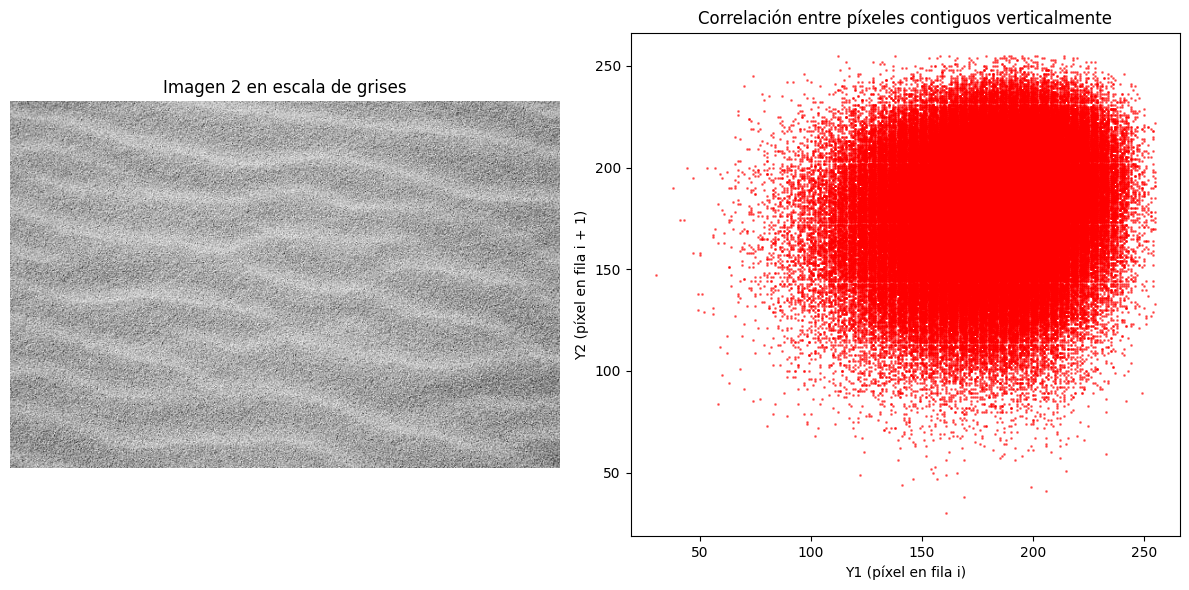
\includegraphics[width=1\textwidth]{Ejercicio1b.png}
    \ \caption{Gráfico de dispersión de la correlación de píxeles contiguos verticalmente de la imagen 2. 
    Se observa que los puntos se encuentran dispersos. Es lo que esperabamos ya que los colores de los pixeles
    vecinos no son similares.}
    \captionsetup{belowskip=0pt}
    \label{fig:correlacion2}
\end{figure}
A diferencia del gráfico anterior, los puntos se encuentran más dispersos, implicando una correlación más baja que la imagen anterior.
Atribuimos la diferencia al ruido perteneciente a esta imagen, y a la falta de suavidad. Los colores entre los píxeles vecinos no están relacionados.

Luego, se estimó el coeficiente de correlación de cada vector. Los resultados son los presentados a continuación:
\begin{enumerate}
    \item Para la Imagen 1 se obtuvo, 
    coeficiente de correlación = 0.9789354535355658

    \item Para la Imagen 2 se obtuvo, 
    coeficiente de correlación = 0.1460473239944978
\end{enumerate}

Los resultados de la primera imagen apoyan lo intuido anteriormente, al aproximarse al valor 1, indican una fuerte correlación entre los píxeles.
Con respecto a la segunda imagen, sus resultados también apoyan lo intuido, al acercarse al valor 0.1, demuestra que los píxeles vecinos no están relacionados.

\vspace{1em}

La diferencia entre ambas imágenes nos indica cuál se podría comprimir con mayor calidad. En primer lugar, la imagen 1 al comprimirse, podría eliminar la redundancia entre píxeles vecinos.
Evitando perder la calidad de la imagen. En cambio, en la imagen 2, la falta de redundancia causa la pérdida de calidad al momento de comprimir, ya que se dificulta la predicción de un píxel a partir de su vecino. 

\vspace{1em}

Por último, se pide una transformación que descorrelacione las variables.
Se utiliza la transformación de descorrelación de PCA, (ver Ecuación~\ref{eq:pca})
De esta forma, \(Y\) es la proyección de \(X\) en el espacio de autovectores de \(C_X\).

Nuevamente, se hace uso de un gráfico de dispersión por imagen, dando los siguientes resultados:

\begin{figure}[H]
    \centering
    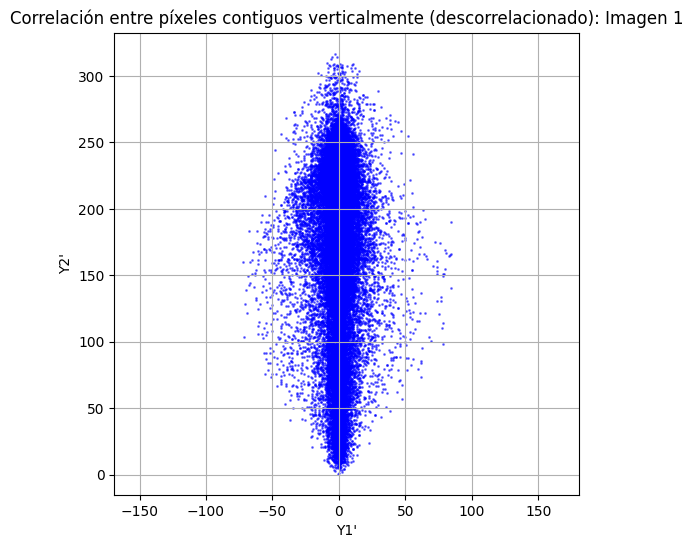
\includegraphics[width=0.7\textwidth]{Ejercicio1c.png}
    \caption{Imagen 1, gráfico de dispersión de la descorrelación de píxeles contiguos verticalmente. Se observa que los píxeles se concentran en el eje vertical Y1, lo que indica que el proceso de descorrelación fue exitoso.}
    \label{fig:descorrelacion1}
\end{figure}
\vspace{-1em}
Podemos observar en la primera imagen cómo los píxeles se encuentran concentrados en el eje vertical Y1, el proceso de descorrelación resulta exitoso.
\vspace{-1em}
\begin{figure}[H]
    \centering
    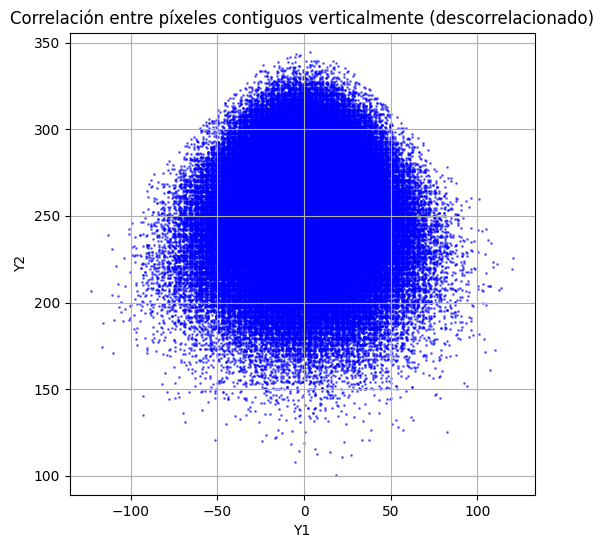
\includegraphics[width=0.7\textwidth]{Ejercicio1d.png}
    \caption{Imagen 2, gráfico de dispersión de la descorrelación de píxeles contiguos verticalmente. El grafico no se concentra entorno a ningun eje, mantiene una forma dispersa.}
    \label{fig:descorrelacion2}
\end{figure}

Por otro lado, en la segunda imagen, el gráfico se mantiene en forma de una nube, como en la Figura 2, demostrando la falta de correlación inicial.
\newpage


\subsection*{Ejercicio 2: Compresión}
\addcontentsline{toc}{subsection}{Ejercicio 2: Compresión}

\vspace{1em}


Para analizar la estructura estadística de los datos, primero se calcula el vector media $\boldsymbol{\mu}$, que contiene el promedio de cada columna de $X$, como se muestra en la Ecuación~\ref{eq:media} de la introducción. Esto se realiza mediante la función \texttt{mean\_estimator()}.

Luego, se centra la matriz de datos restando la media a cada fila, obteniendo así la matriz centrada $X_c$, según la Ecuación~\ref{eq:centrado}. Por como están los datos en la matriz $X$, la media se resta a cada fila, es decir, a cada bloque.

\vspace{1em}



Para aplicar PCA, se utiliza la función \texttt{pca\_transform()}, que resuelve el problema de autovalores y autovectores de la matriz de covarianza, como se define en la Ecuación~\ref{eq:covarianza}. Es decir, se buscan vectores propios y valores propios de $C_X$.

Los autovectores seleccionados se agrupan en la matriz de proyección $P$ (ver Ecuación~\ref{eq:autovectores}), y la proyección de los datos originales sobre este subespacio de menor dimensión se obtiene multiplicando la matriz centrada $X_c$ por $P$, resultando en la matriz $Y$ de datos comprimidos y descorrelacionados, según la Ecuación~\ref{eq:pca}.

El número de componentes $k$ a conservar se determina en función del factor de compresión deseado, y el porcentaje de espacio ahorrado $S$ se calcula como en la Ecuación~\ref{eq:espacio}.

\vspace{1em}


Además, se grafican los autovalores $\lambda_{j}$ para visualizar cuánta información se conserva y cuánta se descarta al reducir la dimensionalidad, utilizando la función \texttt{plot\_eigenvalues()}.


\begin{figure}[H]
    \centering
    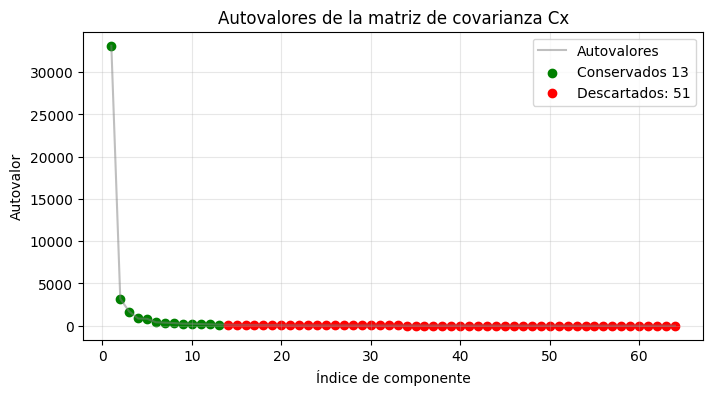
\includegraphics[width=0.7\textwidth]{Ejercicio2.png}
    \caption{Gráfico de dispersión de los autovalores de la matriz de covarianza. En verde se muestran los $k$ autovalores conservados (componentes principales seleccionados) y en rojo los descartados, según el factor de compresión elegido. Se conservan 13 autovalores mientras que se descartan 51}
    \label{fig:eigvals2}
\end{figure}


\newpage
\subsection*{Ejercicio 3: Descompresión}
\addcontentsline{toc}{subsection}{Ejercicio 3: Descompresión}

Luego de lo realizado en el Ejercicio 2, se realiza la reconstrucción de la imagen comprimida utilizando el proceso inverso del PCA de compresión, para descomprimir.
A través del Ejercicio 2, se obtienen los siguientes datos de la imagen:

\vspace{1em}

Vectores \(y_i\) (\(Y\)), la matriz de autovectores (\(P\)) y la media \(\mu_X\) (\(\mu\))

\vspace{1em}

Una vez obtenida la información indicada, se aplica la proyección inversa del PCA para obtener los vectores $x_i$ aproximados, utilizando la Ecuación~\ref{eq:reconstruccion} de la introducción.
De esta manera, obtenemos los siguientes resultados:

\begin{figure}[H]
    \centering
    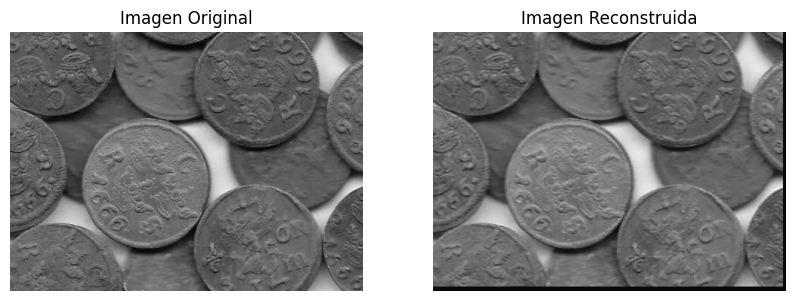
\includegraphics[width=1\textwidth]{Ejercicio3.png}
    \caption{Imagen reconstruida a través del proceso de PCA inverso. Se observan lineas negras en los bordes derecho e inferior, debido a que tomamos bloques de 8x8, mientras que la cantidad de pixeles de la imagen original no es multiplo de 8.}
    \label{fig:ej3}
\end{figure}

Podemos notar el borde negro de la imagen reconstruida, lo cual sucede al no poder completar bloques de exactamente 8 * 8 al comprimir la imagen.
Adicionalmente, podemos observar una diferencia entre las imágenes o pérdida de nitidez, atribuida a la reducción de la dimensionalidad y la eliminación de componentes de menor varianza.

<<<<<<< HEAD
\vspace{0.5em}
=======
\newpage
\section*{Ejercicio 4: Medidas de desempeño}
\addcontentsline{toc}{section}{Ejercicio 4: Medidas de desempeño}
El objetivo de este ejercicio es evaluar el desempeño de la compresión de imágenes al variar el espacio ahorrado (S) (1). 

\vspace{1em}
>>>>>>> bd43e25d04d35a82d222be3772546cd9b3ba1e87

\subsection*{Ejercicio 4: Medidas de desempeño}
\addcontentsline{toc}{subsection}{Ejercicio 4: Medidas de desempeño}

<<<<<<< HEAD
El objetivo de este ejercicio es evaluar el desempeño de la compresión de imágenes al variar el espacio ahorrado $S$, definido en la Ecuación~\ref{eq:espacio}.

En primer lugar, para cada porcentaje de espacio ahorrado comprimimos una imagen y la reconstruimos.

\begin{figure}[H]
    \centering
    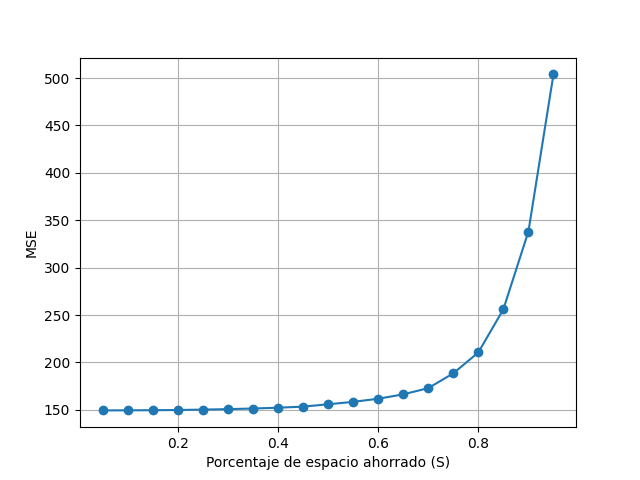
\includegraphics[width=0.6\textwidth]{Ejercicio 4a.png}
    \caption{Gráfico de MSE vs el espacio ahorrado. En el grafico, se observa que el errror cuadratico medio aumenta a 
    medida que lo hace el espacio ahorrado. Este resultado es coherente ya que al descartar un mayor numero de componentes principales, 
    se pierde mas informacion de la imagen.}
    \label{fig:ej4}
\end{figure}

En el gráfico, se observa que el error cuadrático medio (MSE), calculado según la Ecuación~\ref{eq:mse}, aumenta a medida que lo hace el espacio ahorrado.
Sin embargo, esta relación no es proporcional: el error crece considerablemente a partir de un espacio ahorrado del 80\%. Al superar ese porcentaje, la pérdida de información se vuelve significativa, impactando notablemente en la calidad de la imagen. 
=======
\vspace{1em}

En primer lugar, para cada porcentaje de espacio ahorrado comprimimos una imagen y la reconstruimos. Luego, para 
medir el rendimiento del procedimiento, calculamos el error cuadrático medio (MSE) (2) entre la imagen original y 
la reconstruida. 

\vspace{1em}

\begin{equation}
MSE = \frac{1}{N_w N_h} \sum_{i=1}^{N_w} \sum_{j=1}^{N_h} (p_{ij} - \hat{p}_{ij})^2
\end{equation}

\begin{figure}[H]
    \centering
    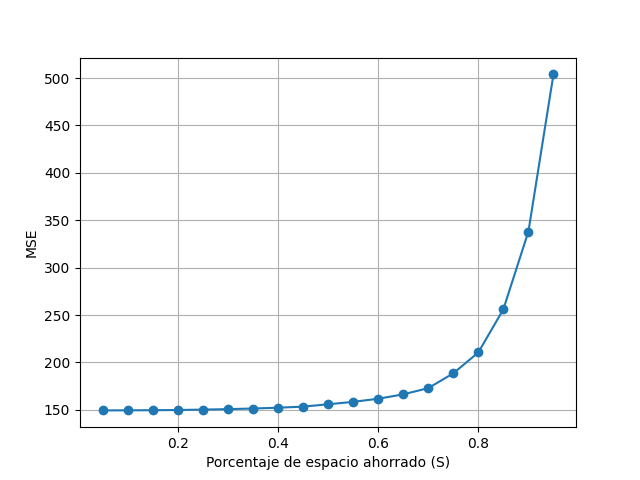
\includegraphics[width=1\textwidth]{Ejercicio 4a.png}
    \caption{Relación entre el MSE y el porcentaje de espacio ahorrado.}
    \label{fig:ej4}
\end{figure}

En el gráfico, se observa que el error cuadrático medio aumenta a medida que lo hace el espacio ahorrado.
Este resultado es coherente, ya que al descartar un mayor número de componentes principales se pierde más 
información de la imagen.
Sin embargo, esta relación no es proporcional: el error crece considerablemente a partir de un espacio 
ahorrado del 80\%. Al superar ese porcentaje, la pérdida de información se vuelve significativa, 
impactando notablemente en la calidad de la imagen. 

\vspace{1em}
>>>>>>> bd43e25d04d35a82d222be3772546cd9b3ba1e87

Para ilustrarlo, incluimos algunas imágenes para diferentes porcentajes de espacio ahorrado. 
\begin{figure}[H]
    \centering
    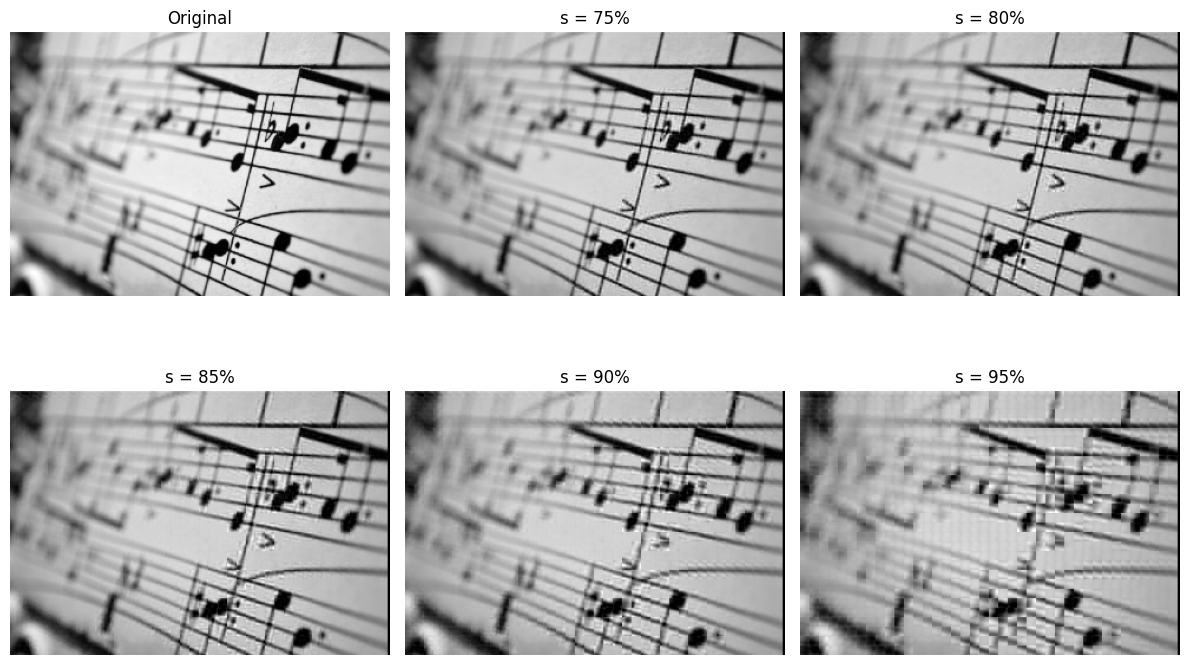
\includegraphics[width=0.95\textwidth]{Ejercicio 4b.png}
    \caption{Imagen original vs las reconstruidas para diferentes S. Las imagenes van perdiendo nitidez a medida que aumenta el porcentaje de espacio ahorrado.}
    \label{fig:ej4b}
\end{figure}

Vemos que a medida que S aumenta, la imagen reconstruida pierde nitidez. La reducción de 
componentes principales se ve en una disminución de la calidad de la imagen. 

\newpage
\subsection*{Conclusiones}
\addcontentsline{toc}{subsection}{Conclusiones}
En este trabajo práctico implementamos y evaluamos la compresión de imágenes usando 
PCA (Análisis de Componentes Principales). Este permite reducir la dimensión de los datos
al descartar las componentes de menor varianza, quedándose con las componentes principales, 
es decir aquellas necesarias para la comprensión de la imagen. De esta manera, se ahorra espacio 
sin comprometer significativamente la calidad de la imagen.

\vspace{1em}

Los resultados mostraron que, a medida que aumenta el porcentaje de espacio ahorrado, la calidad
de la imagen reconstruida decae progresivamente, especialmente a partir de la reducción de 80\%. 
Esto se refleja en un incremento notable del MSE. Sin embargo, consideramos que
para valores intermedios de compresión (cercanos al 70\%), obtenemos un buen balance entre nitidez 
de la imagen y reducción de memoria. 

\vspace{1em}

Los problemas a lo largo de este trabajo práctico fueron mínimos, consistindo principalmente en 
la eleccion de funciones de librerías para el cálculo de autovalores y autovectores, y en la 
implementación de las funciones de compresión y descompresión. Por lo que se tuvo que comprender 
el formato de los datos con los que trabajan estas librerías, llevando lo teorico a la práctica.

\vspace{1em}

En conclusión, la aplicación de PCA para la compresión de imágenes nos permitió observar
de primera mano cómo la reducción de dimensionalidad ayuda en el ahorro de almacenamiento,
sin comprometer demasiado la calidad de la imagen.

\end{document}
